\begin{XeClass}{Trash}
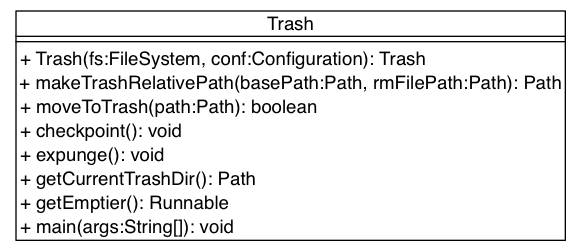
\includegraphics[width=10cm]{cdig/Trash.png}
     
 本类提供了trash机制。文件在删除时会被移动到用户的trash文件夹下,这个文件夹
 位于每个用户的home文件夹下,名字为\emph{.Trash}。
 
 文件被删除时,会先在Trash文件夹下建一个子目录Current,被删除的文件将会将会被
 移动到Current目录下的与原目录相同的目录,比如说
 文件\emph{/user/admin/test/input.in}在被删除后,
 将会被移动到\emph{/user/admin/.Trash/Current/user/admin/test/input.in}。
 
 配置文件中,\emph{fs.trash.interval}可以设置的CheckPoint的时间间隔,
 如果为0,则会禁用trash机制。系统在每个CheckPoint,会将目前\emph{.Trash}
 目录中的\emph{Current}文件夹命名为当前的CheckPoint值,例如
 \emph{/user/admin/.Trash/1507022014/user/admin/test/input.in},
 然后,在下一个CheckPoint,系统将会将所有的超时的CheckPoint彻底删除。
 
 这种设计的优点在于,不用在垃圾管理时遍历要管理的内容,而且不需要文件系统支持
 在文件上设置时间,不用同步时钟。

    \begin{XeMethod}{\XePublic}{Trash}{Trash}
         
 Trash类的构造函数,通过给入FileSystem对象fs和Configuration对象conf
 对Trash类中的静态变量进行初始化。

    \end{XeMethod}

    \begin{XeMethod}{\XePrivate}{Path}{makeTrashRelativePath}
         
 返回要被删除文件目录与垃圾回收站的源目录组合的地址

    \end{XeMethod}

    \begin{XeMethod}{\XePublic}{boolean}{moveToTrash}
         
 移动一个文件或者文件夹到当前的垃圾箱中。此方法会在文件已经存在于垃圾桶
 或者垃圾桶被禁用时返回false

    \end{XeMethod}

    \begin{XeMethod}{\XePublic}{void}{checkpoint}
         
 创建一个CheckPoint.

    \end{XeMethod}

    \begin{XeMethod}{\XePublic}{void}{expunge}
         
 删除过期的CheckPoint.

    \end{XeMethod}

    \begin{XeMethod}{}{Path}{getCurrentTrashDir}
         
 获得当前Trash的工作目录

    \end{XeMethod}

    \begin{XeMethod}{\XePublic}{Runnable}{getEmptier}
         
 返回一个\emph{Runnable}对象,即\emph{org.apache.hadoop.fs.Trash.Emptier.},
 这个对象周期性地清理所有用户的垃圾箱,需要被管理员运行。
 在同一时间,只会在垃圾箱中保留一个CheckPoint

    \end{XeMethod}

    \begin{XeMethod}{\XePublic}{void}{main}
         
 获取Emptier对象并调用其run方法运行

    \end{XeMethod}

    \begin{XeInnerClass}{Emptier}
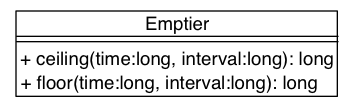
\includegraphics[width=10cm]{cdig/Emptier.png}
         
 该类会独自开一个线程运行,其目的是周期性地对垃圾箱进行清空.

        \begin{XeMethod}{\XePrivate}{long}{ceiling}
             
 将时间间隔的值向上取整

        \end{XeMethod}

        \begin{XeMethod}{\XePrivate}{long}{floor}
             
 将时间间隔的值向下取整

        \end{XeMethod}

    \end{XeInnerClass}
\end{XeClass}
